\documentclass[10pt,twocolumn]{article}
\topmargin=0.0in %length of margin at the top of the page (1 inch added by default)
\oddsidemargin=0.0in %length of margin on sides for odd pages
\evensidemargin=0in %length of margin on sides for even pages
\textwidth=6.5in %How wide you want your text to be
\marginparwidth=0.5in
\headheight=0pt %1in margins at top and bottom (1 inch is added to this value by default)
\headsep=0pt %Increase to increase white space in between headers and the top of the page
\textheight=9.1in %How tall the text body is allowed to be on each page

\usepackage{url}
\usepackage{graphicx}
\usepackage{authblk}
\usepackage{hyperref}

\widowpenalty=500
\clubpenalty=500
\setlength{\parskip}{3pt}

\date{}

\begin{document}

\title{ADAM: Genomics Formats and Processing Patterns for Cloud Scale Computing}
\author[1]{Matt~Massie}
\author[1]{Frank~Austin~Nothaft}
\author[1,2]{Chris~Hartl}
\author[1]{Christos~Kozanitis}
\author[1]{David~Patterson}
\affil[1]{Department of Electrical Engineering and Computer Science, University of California, Berkeley}
\affil[2]{The Broad Institute of MIT and Harvard}

\maketitle

\raggedbottom

\abstract

Current genomics applications are dominated by the movement of data to and from disk. This data movement pattern
is a significant bottleneck that prevents these applications from scaling well to distributed computing clusters. In this report,
we introduce a new set of data formats and programming patterns for genomics applications using in-memory MapReduce
frameworks. These formats improve application performance, data storage efficiency, and programmer productivity.

\section{Introduction}
\label{sec:introduction}

Although the cost of data processing has not historically been an issue for genomic studies, the falling cost of genetic
sequencing will soon turn computational tasks into a dominant cost~\cite{nhgri}. The process of transforming reads
from alignment to variant-calling ready reads involves several processing stages including duplicate marking, base
score quality recalibration, and local realignment. Currently, these stages have involved reading a Sequence/Binary
Alignment Map~(SAM/BAM) file, performing transformations on the data, and writing this data back out to disk as a
new SAM/BAM file~\cite{li09}.

Because of the amount of time these transformations spend shuffling data to and from disk, these transformations have become
the bottleneck in modern variant calling pipelines. It currently takes three days to perform these transformations on a high
coverage BAM file\footnote{A 250GB BAM file at 30$\times$ coverage. See~\S\ref{sec:applications} for a longer discussion}. By
rewriting these applications to make use of modern in-memory MapReduce frameworks like Spark~\cite{zaharia10}, these
transformations can now be completed in FIXME\footnote{FIXME} hours.

In this paper, we introduce ADAM, which is a programming framework and a set of data formats for cloud scale genomic
processing. These frameworks and formats scale efficiently to modern cloud computing performance, which allows us to
parallelize read translation steps that are required between alignment and variant calling. In this paper, we provide an
introduction to the data formats~(\S\ref{sec:current-genomics-storage-standards}) and pipelines used to process
genomes~(\S\ref{sec:genomic-processing-pipelines}), introduce the ADAM formats and data access
application programming interfaces~(APIs)~(\S\ref{sec:data-format-and-api}) and programing
model~(\S\ref{sec:in-memory-programming-model}). Finally, we review the performance and compression gains we
achieve~(\S\ref{sec:performance}), and outline future enhancements to ADAM that we are working on~(\S\ref{sec:future-work}).

Performance teasers.

\section{Current Genomics Storage Standards}
\label{sec:current-genomics-storage-standards}

The current de facto standard for the storage and processing of genomics data in read format is BAM. BAM is a binary file
format that implements the SAM standard for read storage~\cite{li09}. BAM files can be operated on in several languages,
using either the SAMtools~(\cite{li09}, C++), Picard~(\cite{picard}, Java), and Hadoop-BAM~(\cite{niemenmaa12}, Hadoop
MapReduce through Java) APIs. BAM provides efficient access and compression over the SAM file format, as its binary
encoding reduces several fields into a single byte, and eliminates text processing on load. However, the file format has been
criticized as it is difficult to process --- the three main APIs that implement the format each note that they do not fully implement
the format due to its complexity. Additionally, the file format is difficult to use in multiprocessing environments due to its use
of a centralized header; the Hadoop-BAM implementation notes that it's scalability is limited to distributed processing
environments of less than 8 machines.

In response to the growing size of sequencing files\footnote{High coverage BAM files can be approximately 250 GB for a human genome.},
a variety of compression methods have come to light~\cite{kozanitis2011, fritz11, WanBioinformatics, Popitsch2012, Asnani2012, CoxBW, 
recoil, Jones2012, Janin2013}. Slimgene~\cite{kozanitis2011}, cSRA~\cite{SRA}, and CRAM~\cite{fritz11} use reference based compression
techniques to losslessly represent reads while they advocate in favor of lossy quality value representations. The former two use lower
quantization levels to represent quality values and CRAM uses user defined budgets to store only fractions of a quality string. 
In the same spirit, Illumina presented recently a systematic approach of quality score removal in~\cite{Janin2013} which safely ignores
quality scores from predictable nucleotides; these are bases that always appear after certain words. It is also worth mentioning that the
standard configurations of cSRA and CRAM discard the optional fields of the BAM format and also simplify the QNAME field. 

\section{Genomic Processing\\Pipelines}
\label{sec:genomic-processing-pipelines}

After sequencing and alignment, there are a few common steps in modern genomic processing pipelines for producing
variant call ready reads. These steps minimize the amount of erroneous data in the input read set by eliminating duplicate data,
verifying the alignment of short inserts/deletions~(indels), and calibrating the quality scores assigned to bases~(base quality score
recalibration, BQSR). The typical pipeline for variant calling is illustrated in figure~\ref{fig:pipeline}.

\begin{figure}[h]
\begin{center}
\includegraphics[width=0.9\linewidth]{pipeline.pdf}
\end{center}
\caption{Variant Calling Pipeline}
\label{fig:pipeline}
\end{figure}

Traditionally, bioinformaticians have focused on improving the accuracy of the algorithms used for alignment and variant
calling. There is obvious merit to this approach~---~these two steps are the dominant contributors to the accuracy of the variant
calling pipeline. However, the intermediate read processing stages are responsible for the majority of execution time. A
breakdown of stage execution time is shown in table~\ref{tab:stage-time} for the version 2.7 of the Genome Analysis
Toolkit~(GATK), a popular variant calling pipeline~\cite{mckenna10}. The numbers in the table are derived from running on
the NA12878 high-coverage human genome.

\begin{table}[h]
\caption{Processing Stage Times for GATK Pipeline}
\label{tab:stage-time}
\begin{center}
\begin{tabular}{| l | c | c |}
\hline
\bf Stage & \bf GATK 2.7/NA12878 \\
\hline
Alignment & 52 hr \\
Sort & \\
Mark Duplicates & 13 hr \\
BQSR & 6 hr \\
Realignment & 33 hr \\
Call Variants & 4 hr \\
\bf Total & \bf 67 hr \\
\hline
\end{tabular}
\end{center}
\end{table}

To provide the readers with a background about how the stages of this pipeline work, we will discuss the algorithms that
implement the intermediate read processing stages. For a detailed discussion of these algorithms, we refer readers to DePristo
et al~\cite{depristo11}.

\paragraph{Sorting:}
\label{sec:sorting}

This phase performs a pass over the reads and sorts them by the reference position at the start of their alignment.

\paragraph{Duplicate Removal:} 
\label{sec:duplicate-removal}

Due to imperfections during the sequencing process, an unknown number of reads are optically duplicated. If these duplicate
reads are not removed, they will then incorrectly bias the variant caller, and can lead to incorrect variant calls. In this stage, we
review all reads mapped at a specific loci, and discard reads that have identical sequence information.

\paragraph{Base Quality Score Recalibration:} 
\label{sec:bqsr}

During the sequencing process, systemic errors occur that lead to the incorrect assignment of base quality scores. In this step, a
statistical model of the quality scores is built and is then used to revise the measured quality scores.

\paragraph{Local Realignment:} 
\label{sec:local-realignment}

For performance reasons, all modern aligners use algorithms that provide approximate alignments. This can cause reads with
evidence of indels to have slight misalignments with the reference. In this stage, we use fully accurate sequence alignment
methods~(Smith-Waterman algorithm~\cite{smith81}) to locally realign reads that contain evidence of short indels. This pipeline
step is omitted in some variant calling pipelines, if the variant calling algorithm that is implemented is not susceptible to these
local alignment errors.

For current implementations of these read processing steps, performance is limited by disk bandwidth. This is because the operations
read in a SAM/BAM file, perform a bit of processing, and write the data to disk as a new SAM/BAM file. We address this by performing
our processing iteratively in memory. The four read processing stages can then be chained together, eliminating three dumps to
disk and an additional three long reads from disk. 

\section{Design Philosophy}
\label{sec:design-philosophy}

Modern bioinformatics pipelines have been designed without a model for how the system should grow or for how
components of the analytical system should connect. We seek to provide a more principled model for system composition.
Our system architecture was inspired heavily by the Open Systems Interconnection (OSI) model for networking
services~\cite{zimmermann80}. This conceptual model standardized the internal functionality of a networked
computer system, and its "narrow waisted" design was critical to the development of the services that would
become the modern internet. We present a similar decomposition of services for genomics data in
figure~\ref{fig:stack-model}.

\begin{figure}[h]
\begin{center}
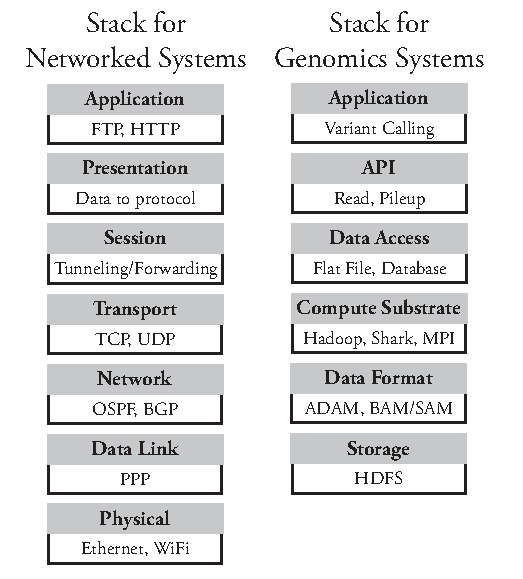
\includegraphics[width=0.9\linewidth]{stack-model.pdf}
\end{center}
\caption{Stack Models for Networking and Genomics}
\label{fig:stack-model}
\end{figure}

The seven levels of our stack model are decomposed as follows:

\begin{enumerate}
\item {\bf Physical Storage:} This layer coordinates data writes to physical media.
\item {\bf Storage:} This layer manages access, replication, and distribution of the genomics files that have been written to disk.
\item {\bf Materialized Data:} This layer encodes the patterns for how data is encoded and stored. This provides read/write efficiency
and compression.
\item {\bf Data Schema:} This level specifies the representation of data when it is accessed, and forms the narrow waist of the pipeline.
\item {\bf Evidence Access:} This layer implements efficient methods for performing common access patterns such as random database
queries, or sequentially reading records from a flat file.
\item {\bf Presentation:} The presentation layer sits on top of the data access layer and provides the application developer with efficient and
straightforward methods for querying the characteristics of individual portions of genetic data.
\item {\bf Application:} Applications like variant calling and alignment are implemented in this layer.
\end{enumerate}

A well defined software stack has several significant advantages. By limiting application interactions with layers lower than the API,
application developers are given a clear and consistent view of the data they are processing. By divorcing the API from the data
access layer, we unlock significant flexibility. With careful design in the data format and data access layers, we can seamlessly
support conventional flat file access patterns, while also allowing easy access to data with database
methods~(see~\S\ref{sec:database-integration}). By treating the compute substrate and storage as separate layers, we also
drastically increase the portability of the APIs that we implement. This approach is a significant improvement over current approaches
which intertwine all layers together --- if all layers are intertwined, new APIs must be developed to support new compute
substrates~\cite{niemenmaa12}, and new access patterns must be carefully retrofitted to the data format that is in use~\cite{kozanitis13}.

We can distill our philosophy into a simple set of goals that drives our design decisions:

\begin{enumerate}
\item TBA.
\end{enumerate}

In the next few sections, we discuss the implementation of ADAM, and how it was designed to satisfy these goals. We then
analyze the performance of our system and discuss the greater impact of our design philosophy.

\section{Data Format and API}
\label{sec:data-format-and-api}

ADAM contains formats for storing read and reference oriented sequence information, and variant/genotype data.
The read oriented sequence format is forwards and backwards compatible with BAM/SAM, and the variant/genotype
data is forwards and backwards compatible with VCF. In this section, we discuss the frameworks used to store this
data. We then introduce the representations, and discuss the content of each representation.

The data representation for the ADAM format is described using the open source Apache Avro data serialization
system~\cite{avro}. The Avro system also provides a human readable schema description language that can
auto-generate the schema implementation in several common languages including Scala, Java, C/C++/C\#,
Python, Ruby, and php. This provides a significant cross-compatibility advantage over the BAM/SAM format,
where the data format has only been implemented for C/C++ through Samtools and for Java through
Picard~\cite{li09,picard}.

We layer this data format inside of the Parquet column store~\cite{parquet}. Parquet is an open source columnar storage
format that was designed by Twitter, which can be used as a single flat file, a distributed file, or as a database inside of
Hive, Shark, or Impala. Columnar stores like Parquet provide several significant advantages when storing genomic data:

\begin{itemize}
\item Column stores enable predicate pushdown~\cite{lamb12}, which minimizes the amount of data read from disk. When
using predicate pushdown, we deserialize specific fields in a record from disk, and apply them to a predicate function. We
then only read the full record if it passes the predicate. This is useful when implementing filters that check read quality.
\item Column stores achieve extremely high compression~\cite{abadi06}. This reduces storage space on disk, and also improves
serialization performance inside of MapReduce frameworks. We are able to achieve a 0.75$\times$ lossless compression
ratio when compared to BAM, and have especially impressive results on quality scores. This is discussed in more
detail in~\S\ref{sec:compression}.
\item Varied data projections can be achieved with column stores. This means that we can choose to only read several
fields from a record. This improves performance for applications that do not read all the fields of a record. Additionally,
we do not pay for null fields in records that we store. This allows us to easily implement lossy compression on top of the
ADAM format, and also allows us to eliminate the FASTQ standard.
\end{itemize}

By supporting varied data projections with low cost for field nullification, we can implement lossy compression on top
of the ADAM format. We discuss this further in~\S\ref{sec:compression}.

A visualization of how ADAM in Parquet compares with BAM can be seen in figure~\ref{fig:file-format}. We remove the file header
and instead distribute these values across all of the records stored. This eliminates global information and makes the file much
simpler to distribute across machines. This is effectively free in a columnar store, as the store just notes that the information is
replicated across many reads. Additionally, Parquet writes data to disk in regularly sized row groups~(from~\cite{parquet}, see
Parquet format readme)~---~this allows parallelism across rows by enabling the columnar store to be split into independent
groups of reads.

\begin{figure}[h]
\begin{center}
\includegraphics[width=\linewidth]{file-format.pdf}
\end{center}
\caption{Comparative Visualization of BAM and ADAM File Formats}
\label{fig:file-format}
\end{figure}

As discussed in~\S\ref{sec:design-philosophy}, the internal data types presented in this section make up the narrow waist of our
proposed genomics stack. In~\S\ref{sec:database-integration} and~\S\ref{sec:columnar-vs-row-storage}, we review how this
abstraction allows us to support different data access frameworks and storage techniques to tailor the stack for the needs of
a specific application.

\subsection{Read Oriented Storage}
\label{sec:read-oriented-storage}

Our default read oriented data format is defined in table~\ref{tab:read-oriented-format}. This format provides all of the
fields supported by the SAM format. To make it easier to split the file between multiple machines for distributed processing,
we have eliminated the file header. Instead, the data encoded in the file header can be reproduced from every single
record. Because our columnar store supports dictionary encoding and these fields are replicated across all records,
replicating this data across all records has a negligible cost in terms of file size on disk.

\begin{table}[h]
\caption{Read Oriented Format}
\label{tab:read-oriented-format}
\begin{center}
\begin{tabular}{| c | l | c |}
\hline
\bf Group & \bf Field & \bf Type \\
\hline
General & Reference Name & String \\
 & Reference ID & Int \\
 & Start & Long \\
 & Mapping Quality & Int \\
 & Read Name & String \\
 & Sequence & String \\
 & Mate Reference & String \\
 & Mate Alignment Start & Long \\
 & Mate Reference ID & Int \\
 & Cigar & String \\
 & Base Quality & String \\
\hline
Flags & Read Paired & Boolean \\
 & Proper Pair & Boolean \\
 & Read Mapped & Boolean \\
 & Mate Mapped & Boolean \\
 & Read Negative Strand & Boolean \\
 & Mate Negative Strand & Boolean \\
 & First Of Pair & Boolean \\
 & Second Of Pair & Boolean \\
 & Primary Alignment & Boolean \\
 & Failed Vendor Checks & Boolean \\
 & Duplicate Read & Boolean \\
\hline
Attributes & Mismatching Positions & String \\
 & Other Attributes & String \\
\hline
Read Group & Sequencing Center & String \\
 & Description & String \\
 & Run Date & Long \\
 & Flow Order & String \\
 & Key Sequence & String \\
 & Library & String \\
 & Median Insert & Int \\
 & Platform & String \\
 & Platform Unit & String \\
 & Sample & String \\
\hline
\end{tabular}
\end{center}
\end{table}

This format is used to store all data on disk. In addition to this format, we provide an enhanced API for accessing read
data.

\subsection{Reference Oriented Storage}
\label{sec:reference-oriented-storage}

In addition to storing sequences as reads, we provide a storage format for reference oriented (pileup) data. This format
is documented in table~\ref{tab:reference-oriented-format}. This pileup format is also used to implement a data storage
format similar to the GATK's ReducedReads format~\cite{depristo11}.

\begin{table}[h]
\caption{Reference Oriented Format}
\label{tab:reference-oriented-format}
\begin{center}
\begin{tabular}{| c | l | c |}
\hline
\bf Group & \bf Field & \bf Type \\
\hline
General & Reference Name & String \\
 & Reference ID & Int \\
 & Position & Long \\
 & Range Offset & Int \\
 & Range Length & Int \\
 & Reference Base & Base \\
 & Read Base & Base \\
 & Base Quality & Int \\
 & Mapping Quality & Int \\
 & Number Soft Clipped & Int \\
 & Number Reverse Strand & Int \\
 & Count At Position & Int \\
\hline
Read Group & Sequencing Center & String \\
 & Description & String \\
 & Run Date & Long \\
 & Flow Order & String \\
 & Key Sequence & String \\
 & Library & String \\
 & Median Insert & Int \\
 & Platform & String \\
 & Platform Unit & String \\
 & Sample & String \\
\hline
\end{tabular}
\end{center}
\end{table}

We treat inserts as an inserted sequence range at the locus position. For bases that are an alignment match against the
reference\footnote{Following the conventions for CIGAR strings, an alignment match does not necessarily correspond to
a sequence match. An alignment match simply means that the base is not part of an indel. The base may not match the
reference base at the loci.}, we store the read base and set the range offset and length to 0. For deletions, we perform the
same operation for each reference position in the deletion, but set the read base to null. For inserts, we set the range length
to the length of the insert. We step through the insert from the start of the read to the end of the read, and increment the
range offset at each position.

As noted earlier, this datatype supports an operation similar to the GATK's ReducedRead datatype. We refer to these datatypes
as aggregated pileups. We perform aggregation by grouping together all bases that share a common reference position and
read base. Within an insert, we group further by the position in the insert. Once the bases have been grouped together, we average
the base and mapping quality scores. We also count the number of soft clipped bases that show up at this location, and the amount
of bases that are mapped to the reverse strand.

\subsection{Variant and Genotype Storage}
\label{sec:variant-and-genotype-storage}

Chris H.

\begin{table}[h]
\caption{Genotype Format}
\label{tab:genotype-format}
\begin{center}
\begin{tabular}{| l | c |}
\hline
\bf Field & \bf Type \\
\hline
Sample ID & String \\
Genotype & Array[Int] \\
Likelihood (Phred) & Array[Int] \\
Format & String \\
\hline
\end{tabular}
\end{center}
\end{table}

\begin{table}[h]
\caption{Variant Format}
\label{tab:variant-format}
\begin{center}
\begin{tabular}{| l | c |}
\hline
\bf Field & \bf Type \\
\hline
Reference Name & String \\
Position & Long \\
Variant ID & String \\
Reference Allele & String \\
Alternate Alleles & Array[String] \\
Allele Count & Array[Int] \\
Chromosome Count & Int \\
Type & Variant Type \\
Info & String \\
Filter & String \\
Genotypes & Array[AdamGenotype] \\
\hline
\end{tabular}
\end{center}
\end{table}

Variant type is one of SNP, multiple nucleotide polymorphism~(MNP), insertion, deletion, structural variant~(SV), or complex.

\section{In-Memory Programming\\Model}
\label{sec:in-memory-programming-model}

As discussed in~\S\ref{sec:genomic-processing-pipelines}, the main bottleneck in current genomics processing pipelines is
packaging data up on disk in a BAM file after each processing step. While this process is useful as it maintains data
lineage\footnote{Since we store the intermediate data from each processing step, we can later redo all pipeline processing
after a certain stage without needing to rerun the earlier stages. This comes at the obvious cost of space on disk. This tradeoff
makes sense if the cost of keeping data on disk and reloading it later is lower than the cost of recomputing the data. This
does not necessarily hold for modern MapReduce frameworks~\cite{zaharia12}.}, it significantly increases the latency of the
processing pipeline.

For the processing pipeline we have built on top of the ADAM format, we have minimized disk accesses~(read one file at the
start of the pipeline, and write one file after all transformations have been completed). Instead, we cache the reads that we are
transforming in memory, and chain multiple transformations together. Our pipeline is implemented on top of the Spark MapReduce
framework, where reads are stored as a map using the Resilient Distributed Dataset~(RDD) primitive.

\section{Performance}
\label{sec:performance}

\subsection{Microbenchmarks}
\label{sec:microbenchmarks}

To validate the performance of ADAM, we created several microbenchmarks. These microbenchmarks are meant to demonstrate
the pure read/write throughput of ADAM, and to show how the system scales in a cluster. To validate these benchmarks, we implemented
the relevant tests in both ADAM and Hadoop-BAM~\cite{niemenmaa12}, running on Spark on an Amazon Elastic Compute 2 (EC2)
cluster. We used the $m2.4xlarge$ instance type for all of our tests. This instance type is an 8 core memory optimized machine
with 68.4 Gibibytes (GiB) of memory per machine. We ran these benchmarks against two genomes from the 1000 Genomes project:
HG00096, a low-coverage human genome (15 GB BAM), and NA12878, a high-coverage human genome (246 GB BAM).

\subsubsection{Read Length and Quality:} 
\label{sec:read-length-and-quality}

This microbenchmark scans all the reads in the file, and collects statistics about the length of the read, and the mapping quality score.
The results of this benchmark can be found in Figure~\ref{fig:length-quality}.

\begin{figure}[h]
\begin{center}
\includegraphics[width=\linewidth]{microbenchmarks/length_and_quality_low_coverage.pdf}
\end{center}
\label{fig:length-quality}
\end{figure}

\subsection{Applications}
\label{sec:applications}

Matt (Sort/MarkDup) and Chris H (BQSR)

\subsection{Compression}
\label{sec:compression}

Frank

\section{Future Work}
\label{sec:future-work}

Beyond the initial release of the ADAM data formats, API, and read transformations, we are working on several other
extensions to ADAM. These extensions strive to make ADAM accessible to more users and to more programming patterns.

\subsection{Database Integration}
\label{sec:database-integration}

ADAM format plays a central role in a library that we develop which will allow sequencing data to be queried from 
the popular SQL based warehouse software such as Shark~\cite{shark}, Hive~\cite{hive} and Impala~\cite{impala}. In fact,
the Avro/Parquet storage backend enables the direct usage of ADAM files as SQL tables; this integration is facilitated through libraries 
that integrate Parquet with the aforementioned software~\cite{parquet}.

Of course there is a lot of work remaining before SHARK provides biologically relevant functionality,
such as the one that is outlined in Bafna et al~\cite{bafna2013}; Shark needs to be enhanced with libraries that provide
efficient indexing, storage management and interval query handling. The indexing scheme that we develop enables
range based read retrieval, such as the indexing mechanism of samtools, quick access to mate pair reads such as the
indexing mechanism of GQL~\cite{kozanitis13} and also text based search features on fields such as the read sequence
and the CIGAR string. To keep storage under control we implement a set of heuristics that prevent the materialization of
queries with reproducible output. Finally, given that most biological data is modelled after intervals on the human genome,
our library includes user defined functions that implement interval operators such as the IntervalJoin operator of GQL.

\subsection{API Support Across Languages}
\label{sec:api-support-across-languages}

Currently, the ADAM API and example read processing pipeline are implemented in the Scala language. However, long
term we plan to make the API accessible to users of other languages. ADAM is built on top of Avro, Parquet, and Spark.
Spark has bindings for Scala, Java, and Python, and Parquet implementations exist for Java and C++. As the data model
is implemented on top of Avro, the data model can also be auto\-generated for C/C++/C\#, Python, Ruby, and php. We hope
to make API implementations available for some of these languages at a later date.

\section{Discussion}
\label{sec:discussion}

Table to go here.

\subsection{Columnar vs. Row Storage}
\label{sec:columnar-vs-row-storage}

In our current implementation, we use the Parquet columnar store to implement the data access layer. We chose to use
columnar storage as we believe that columnar storage is a better fit for bioinformatics workloads than flat row storage;
this discussion is introduced in~\S\ref{sec:data-format-and-api}. Typically, column based storage is preferable unless
our workload is write heavy; write heavy workloads perform better with row based storage formats~\cite{stonebraker05}.
Genomics pipelines tend to skew in favor of reading data~---~pipelines tend to read a large dataset, prune/reduce data,
perform an analysis, and then write out a significantly smaller file that contains the results of the analysis.

However, it is conceivable that emerging workloads could change to be write heavy. We note that although our current
implementation would not be optimized for these workloads, the layered model proposed in~\S\ref{sec:design-philosophy}
allows us to easily change our implementation. Specifically, we can swap out columnar storage in the data access layer with
row oriented storage~\footnote{It is worth noting that the Avro serialization system that we use to define ADAM is a performant
row oriented system.}. The rest of the implementation in the system would be isolated from this change: algorithms in the
pipeline would be implemented on top of the higher level API, and the compute substrate would interact with the data access
layer to implement the process of reading and writing data. 

\subsection{Dancehall vs. Datacenter}
\label{sec:dancehall-vs-datacenter}

Matt

\subsection{New Applications Enabled\\By ADAM}
\label{sec:new-applications}

Chris H (fallback to Frank?)

\subsection{Programming Model\\Improvements}
\label{sec:programming-model-improvements}

Beyond improving performance by processing data in memory, our programming model improves programmer efficiency.
We build our operations as a set of transforms that extend the RDD processing available in Spark. These transformations
allow a very straightforward programming model that has been demonstrated to significantly reduce code size~\cite{zaharia12}.
Additionally, the use of Scala, which is an object functional statically typed language that supports type inference couples
provides further gains.

Additional gains come from our data model. We expose a clear schema, and build an API that expands upon this schema
to implement commonly needed functions. This API represents level 6 in the stack we proposed in
section~\S\ref{sec:design-philosophy}. To reduce the cost of this API, we make any additional transformations from our
internal schema to the data types presented in our API lazy. This eliminates the cost of providing these functions if they are
not used. Additionally, if an additional transformation is required, we only pay the cost the first time the transformation is performed.

In total, these improvements can provide a $2\times$ improvement in programmer productivity. This is demonstrated through
GAParquet, which demonstrates some of the functionality in the GATK on top of the ADAM stack~\cite{gaparquet}. In the
DiagnoseTargets stage of GATK, the number of lines of code~(LOC) needed to implement the stage dropped from 400 to
200. We also see a reduction in lines of code needed to implement the read transformation pipeline described
in~\S\ref{sec:genomic-processing-pipelines}. A LOC comparison of GATK/GAParquet and the read transformation pipeline
is found in table~\ref{tab:lines-of-code}.

\begin{table}[h]
\caption{Lines of Code for ADAM and Original Implementation}
\label{tab:lines-of-code}
\begin{center}
\begin{tabular}{| l | c | c |}
\hline
\bf Application & \bf Original & \bf ADAM \\
\hline
\hline
\multicolumn{3}{| l |}{\bf GATK Diagnose Targets} \\
\hline
Walker & 326 & 134 \\
Subclass & 93 & 66 \\
\bf Total & \bf 419 & \bf 200 \\
\hline
\hline
\multicolumn{3}{| l |}{\bf Translation Pipeline} \\
\hline
BQSR & & \\
Mark Duplicates & & \\
Realign Indels & & \\
Sort & & \\
\bf Total & & \\
\hline
\end{tabular}
\end{center}
\end{table}

\subsection{Benefits of Explicit Schema}
\label{sec:benefits-of-explicit-schema}

Matt

\section{Summary}
\label{sec:summary}

In this technical report, we have presented ADAM which is a new data storage format and processing pipeline for
genomics data. ADAM makes use of efficient columnar storage systems to improve the lossless compression available
for storing read data, and uses in-memory processing techniques to eliminate the read processing bottleneck faced
by modern variant calling pipelines. On top of the file formats that we have implemented, we also present APIs that enhance
developer access to read, pileup, genotype, and variant data. We are currently in the process of extending ADAM to
support SQL querying of genomic data, and extending our API to more programming languages. ADAM promises
to improve the development of applications that process genomic data, by removing current difficulties with the extraction
and loading of data and by providing simple and performant programming abstractions for processing this data.

\section{Availability}
\label{sec:availability}

The ADAM source code is available at Github at \url{http://www.github.com/massie/adam}, and the ADAM project website
is at \url{http://adam.cs.berkeley.edu}. Additionally, ADAM is deployed through Maven with the following dependency:

\begin{verbatim}
TBD
\end{verbatim}

At publication time, the current version of ADAM is 0.5.0. ADAM is open source and is released under the Apache 2
license.

\bibliographystyle{acm}

\bibliography{adam-tr}

\clearpage

\end{document}